%iffalse
\let\negmedspace\undefined
\let\negthickspace\undefined
\documentclass[journal,12pt,onecolumn]{IEEEtran}
\usepackage{cite}
\usepackage{amsmath,amssymb,amsfonts,amsthm}
\usepackage{algorithmic}
\usepackage{graphicx}
\usepackage{textcomp}
\usepackage{xcolor}
\usepackage{txfonts}
\usepackage{listings}
\usepackage{enumitem}
\usepackage{mathtools}
\usepackage{gensymb}
\usepackage{comment}
\usepackage[breaklinks=true]{hyperref}
\usepackage{tkz-euclide} 
\usepackage{listings}
\usepackage{gvv}                                        
%\def\inputGnumericTable{}                                 
\usepackage[latin1]{inputenc}     
\usepackage{xparse}
\usepackage{color}                                            
\usepackage{array}                                            
\usepackage{longtable}                                       
\usepackage{calc}                                             
\usepackage{multirow}
\usepackage{multicol}
\usepackage{hhline}                                           
\usepackage{ifthen}                                           
\usepackage{lscape}
\usepackage{tabularx}
\usepackage{array}
\usepackage{float}
\newtheorem{theorem}{Theorem}[section]
\newtheorem{problem}{Problem}
\newtheorem{proposition}{Proposition}[section]
\newtheorem{lemma}{Lemma}[section]
\newtheorem{corollary}[theorem]{Corollary}
\newtheorem{example}{Example}[section]
\newtheorem{definition}[problem]{Definition}
\newcommand{\BEQA}{\begin{eqnarray}}
\newcommand{\EEQA}{\end{eqnarray}}
\usepackage{float}
\usepackage{listings}
\usepackage{xcolor}
%\newcommand{\define}{\stackrel{\triangle}{=}}
\theoremstyle{remark}
\usepackage{ circuitikz }
%\newtheorem{rem}{Remark}
% Marks the beginning of the document
\begin{document}
\title{10.3.2.5}
\author{EE24BTECH11007 - Arnav Makarand Yadnopavit}
\maketitle
\renewcommand{\thefigure}{\theenumi}
\renewcommand{\thetable}{\theenumi}
\parindent 0px Question: Half the perimeter of a rectangular garden, whose length is 4 m more than its width, is
36 m. Find the dimensions of the garden.\\
\solution\\
Let length and width of the garden be $x$ and $y$ respectively 
\begin{align}
    x+y=36\\
    x-y=4
\end{align}

We represent the system in matrix form:
\begin{align}
A = \myvec{1 & 1 \\ 1 & -1}, \quad
b = \myvec{36 \\ 4}, \quad
x = \myvec{x \\ y}.
\end{align}

\subsection*{LU factorization using update equaitons}
    Given a matrix $ \mathbf{A} $ of size $ n \times n $, LU decomposition is performed row by row and column by column. The update equations are as follows:\\
    \textbf{Step-by-Step Procedure:}\\
1. Initialization: 
   - Start by initializing $ \mathbf{L} $ as the identity matrix $ \mathbf{L} = \mathbf{I} $ and $ \mathbf{U} $ as a copy of $ \mathbf{A} $.
   
2. Iterative Update:
   - For each pivot $ k = 1, 2, \ldots, n $:
     - Compute the entries of $ U $ using the first update equation.
     - Compute the entries of $ L $ using the second update equation.
   
3. Result:
   - After completing the iterations, the matrix $ \mathbf{A} $ is decomposed into $ \mathbf{L} \cdot \mathbf{U} $, where $ \mathbf{L} $ is a lower triangular matrix with ones on the diagonal, and $ \mathbf{U} $ is an upper triangular matrix.

    

\subsection*{1. Update for $ U_{k,j} $ (Entries of $ U $)}

For each column $ j \geq k $, the entries of $ U $ in the $ k $-th row are updated as:
\[
U_{k,j} = A_{k,j} - \sum_{m=1}^{k-1} L_{k,m} \cdot U_{m,j}, \quad \text{for } j \geq k.
\]
This equation computes the elements of the upper triangular matrix $ \mathbf{U} $ by eliminating the lower triangular portion of the matrix.

\subsection*{2. Update for $ L_{i,k} $ (Entries of $ L $)}

For each row $ i > k $, the entries of $ L $ in the $ k $-th column are updated as:
\[
L_{i,k} = \frac{1}{U_{k,k}} \left( A_{i,k} - \sum_{m=1}^{k-1} L_{i,m} \cdot U_{m,k} \right), \quad \text{for } i > k.
\]
This equation computes the elements of the lower triangular matrix $ \mathbf{L} $, where each entry in the column is determined by the values in the rows above it.\\
Using a code we get L,U as 
\begin{align}
L = \myvec{1 & 0 \\ 1 & 1}, \quad
U = \myvec{1 & 1 \\ 0 & -2}.
\end{align}

\subsection*{Solving $A{x} = {b}$}

\subsubsection*{Forward Substitution: Solve $Ly = b$}
\begin{align}
\myvec{1 & 0 \\ 1 & 1}
\myvec{y_1 \\ y_2}
=
\myvec{36 \\ 4}.
\end{align}

From the first row:
\begin{align}
y_1 = 36.
\end{align}

From the second row:
\begin{align}
y_1 + y_2 &= 4 \\
36 + y_2 &= 4 \\
y_2 &= -32.
\end{align}

Thus:
\begin{align}
{y} = \myvec{36 \\ -32}.
\end{align}

\subsubsection*{Back Substitution: Solve $Ux = y$}
\begin{align}
\myvec{1 & 1 \\ 0 & -2}
\myvec{x \\ y}
=
\myvec{36 \\ -32}.
\end{align}

From the first row:
\begin{align}
x + y = 36.
\end{align}

From the second row:
\begin{align}
-2y = -32 \\
y = 16.
\end{align}

Substitute $y = 16$ into the first equation:
\begin{align}
x + 16 = 36 \\
x = 20.
\end{align}

Thus:
\begin{align}
x = 20, \quad y = 16.
\end{align}





\begin{figure}[H]
    \centering
    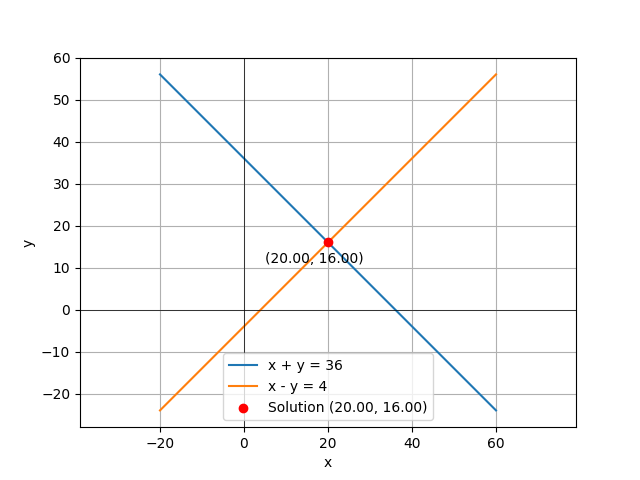
\includegraphics[width=\columnwidth]{figs/fig.png}
 \end{figure}
\end{document}


